\begin{figure}[t]
\centering
\small
\setlength{\tabcolsep}{3pt}
\begin{minipage}[b]{0.5\linewidth}
    \centering
    \begin{tabular*}{\linewidth}{@{\extracolsep{\fill}}lccc@{}}
    \toprule
    \textbf{Filter} & \textbf{\#Trajectories} & \textbf{Test-N} & \textbf{Test-C} \\
    \midrule
    No filtering & 19,464 & 61.4  & 39.2 \\
    \midrule
    GLM-5.1-FP8 & 16,966 & 58.5  & 37.1 \\ 
    \midrule
    Gemini-3.1-Pro & 15,617 & \textbf{64.9} & \textbf{49.1} \\
    \bottomrule
    \end{tabular*}
    \captionof{table}{AppWorld performance of Qwen3-8B trained on ESAT-S52-AW7 data filtered with different judge models.}
    \label{tab:trajectory_filtering}
\end{minipage}
\hfill
\begin{minipage}[b]{0.45\linewidth}
    \centering
    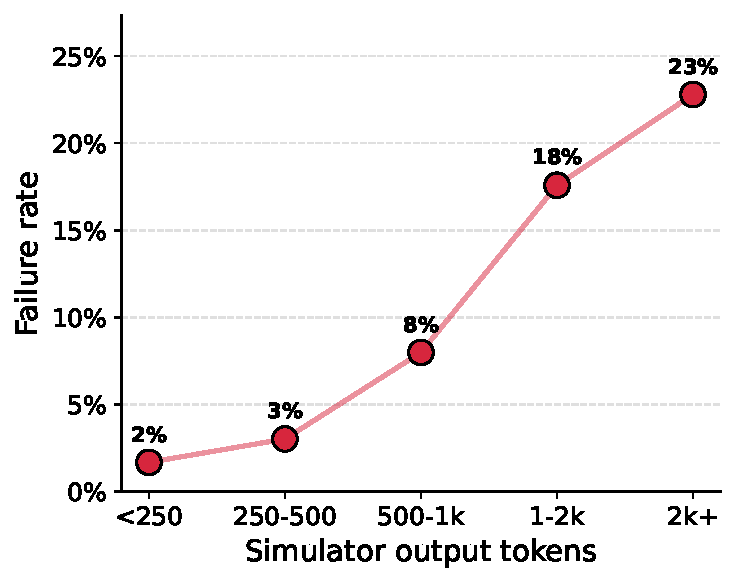
\includegraphics[width=0.8\linewidth]{images/failure_rate_by_output_tokens.pdf}
    \caption{Simulator failure rate as a function of output token length, as judged by GPT-5.1.}
    \label{fig:length}
\end{minipage}
\end{figure}

